% *********************************************************************
% © 2021–2024 Jeremy Sylvestre
%
% Permission is granted to copy, distribute and/or modify this document
% under the terms of the GNU Free Documentation License, Version 1.3 or
% any later version published by the Free Software Foundation; with no
% Invariant Sections, no Front-Cover Texts, and no Back-Cover Texts. A
% copy of the license is included in the appendix entitled “GNU Free
% Documentation License” that appears in the output document of this
% PreTeXt source code. All trademarks™ are the registered® marks of
% their respective owners.
%
% *********************************************************************

\newcommand*{\xmin}{-1.5}
\newcommand*{\xmax}{1.5}
\newcommand*{\ymin}{-1.5}
\newcommand*{\ymax}{1.5}

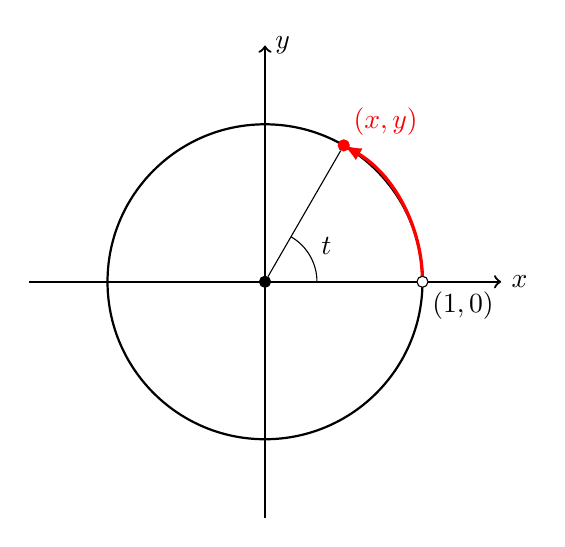
\begin{tikzpicture}
[
	closedpt/.style={circle,draw,fill,inner sep=0pt,minimum size=4pt},
	openpt/.style={circle,draw,inner sep=0pt,minimum size=4pt},
	scale=2
]

	% axes
	\draw[->,thick] (\xmin,0) -- (\xmax,0) node[right] {$x$};
	\draw[->,thick] (0,\ymin) -- (0,\ymax) node[right] {$y$};

	\node[closedpt] at (0,0) (o) {};

	\draw[thick] (1,0) arc (0:360:1cm);
	\draw[-latex,red,very thick] (1,0) arc (0:60:1cm);
	\draw[white,fill=white] (1,0) circle (0.03cm);
	\node[openpt] at (1,0) (r) {};
	\draw[white,fill=white] (0.5,0.866) circle (0.03cm);
	\node[closedpt,red] at (0.5,0.866) (r2) {};
	\node[below right] at (r) {$(1,0)$};
	\node[above right,red] at (r2) {$(x,y)$};

	\draw (o) -- (r2);
	\draw (0.33,0) arc (0:60:0.33cm);
	\node at (0.39,0.225) {$t$};

\end{tikzpicture}
